\documentclass{article}
% Primary A — полный вариант статьи
% Shared NeurIPS-RU two-column preamble (input from paper variants).
\usepackage[preprint]{neurips_2025}

\usepackage{fontspec}
\usepackage{polyglossia}
\setdefaultlanguage{russian}
\setotherlanguage{english}
\setmainfont{Liberation Serif}
\setsansfont{Liberation Sans}
\setmonofont{Liberation Mono}

\usepackage{amsmath,amssymb}
\usepackage{booktabs}
\usepackage{multirow}
\usepackage{graphicx}
\usepackage{url}
\usepackage{hyperref}
\usepackage{xcolor}
\usepackage{microtype}
\usepackage{enumitem}

\graphicspath{{images/}{../mmcs-sfedu_thesis7/images/}}

\makeatletter
\renewcommand{\@notice}{%
  \begingroup
    \renewcommand{\thefootnote}{}%
    \footnotetext[0]{\hspace*{-\parindent}\footnotesize\@noticestring}%
  \endgroup
}
\AtBeginDocument{%
  \newgeometry{%
    letterpaper,%
    textheight=9in,%
    textwidth=7in,%
    top=1in,%
    left=0.75in,%
    headheight=12pt,%
    headsep=25pt,%
    footskip=30pt%
  }%
  \setlength{\columnsep}{0.25in}%
  \setlength{\columnseprule}{0pt}%
}
\makeatother

\newcommand{\rem}{\mathrm{REM}}
\newcommand{\elpd}{\mathrm{elpd}}
\newcommand{\PS}{ПС}


\title{Primary~A: суточное среднее и размах профиля ПС\\
в байесовской модели разладки перед сейсмическим событием}

\author{%
  С.~А.~Пономарёв \\
  Институт математики, механики и компьютерных наук\\
  Южный федеральный университет \\
  \texttt{ponomarev@sfedu.ru} \\
}

\begin{document}

\twocolumn[{%
\maketitle
\begin{abstract}
Фиксируем \emph{заранее} основной (primary) анализ~A конвейера
\texttt{seismic-pipeline}: признаки \texttt{daily:mean+range},
разрешение профиля $N{=}24$, $\mathrm{overlap}{=}0{,}5$
(эквивалент устаревших окон $W{=}2$, $S{=}1$), правдоподобия
Student-$t$ (или normal) для среднего и
\texttt{beta\_constrained} ($\alpha,\beta\ge 1$) для
\emph{размаха профиля ПС}. На страте \texttt{full} ($33$
восьмидневных профиля, включая влиятельные окна $2024$-$09$-$30$)
confirmatory MCMC даёт
$\mathbb{E}[\tau]{=}6{,}285$ суток до события
(ширина HDI$_{60}{=}1{,}342$),
$\overline{\elpd}_{\mathrm{LOO}}/(F E'){=}3{,}034$.
Plain Beta на размахе отвергаем как диагностический артефакт
границы; влиятельные события \emph{не} удаляем из primary, а
отчитываем with/without. Результат --- смена REM-режима, не стресс
и не прогноз землетрясений.

\medskip
\noindent\textbf{Ключевые слова:}
парадоксальный сон, размах профиля ПС, точка разладки, primary-анализ,
PSIS-LOO.
\end{abstract}
\vspace{1.0em}
}]

\section{Введение}

Геофизические предвестники сейсмических событий описаны для
ряда регионов~\cite{Rodkin2011,Cicerone2009}, а поведенческие
аномалии животных перед толчками обсуждаются в биологической
литературе~\cite{Kirschvink2000,Grant2011}. Эти наблюдения
требуют проверки на инструментальных физиологических рядах.

Стресс у грызунов меняет структуру парадоксального
сна~\cite{Rampin1991,Meerlo1997,Sanford2010}. Непрерывная
регистрация ЭКоГ позволяет поставить узкий вопрос: есть ли
смена режима REM-динамики в фиксированном окне до толчка?

Классические нейросейсмоотчёты по той же площадке опирались на
\emph{размах профиля ПС} ($12\times 2$\,ч без перекрытия) и
сообщали эффект в окне $\sim 2$--$4$ суток. Здесь оценивается
иной параметр --- момент \emph{начала} режима $\tau$ в модели
одной разладки на восьми сутках.

На малой выборке полный перебор ($896$ окон $W/S$; $1224$ сеток
$N\times\mathrm{overlap}$) полезен для разведки, но опасен для
выводов: ELPD может раздуваться артефактом likelihood. Поэтому
фиксируем primary-конфиг~\textbf{A} \emph{до} нарратива
ранжирования~\cite{Vehtari2017}. Параллельный вариант~\textbf{B}
(только \texttt{daily:range}) --- отдельная статья.

\section{Данные}

\subsection{Животные и регистрация}

ЭКоГ и активность гиппокампа непрерывно регистрировались у
взрослых самцов крыс на станции ``Институт'' КФ ЕГС РАН
($23\pm1^{\circ}$C, $12$\,ч свет / $12$\,ч темнота; оцифровка
$1$\,кГц). Процедуры одобрены биоэтической комиссией ЮФУ.

\subsection{Гипнограмма}

Суточную запись делят на эпохи $5$\,с. После исключения
артефактов медленный сон определяют по дельта-мощности ЭКоГ
($2{,}5$--$5{,}5$\,Гц), парадоксальный --- по отношению
тета/дельта в гиппокампе~\cite{Fang2010,Vyazovskiy2005,Saevskiy2025}.

\subsection{События и страта primary}

Отобраны даты с интенсивностью $>2$ и доступной гипнограммой.
Каждое окно --- $8$ суток. Направление \texttt{before} ---
пресобытийный ряд; \texttt{after\_reversed} --- послесобытийное
окно, развёрнутое для единого builder'а (биологически ближе к
recovery).

\paragraph{Страта primary~A.}
\texttt{full}: before + after\_reversed, $33$ экспортированных
профиля из $36$ запрошенных. Три неполных after\_reversed
(\texttt{exported=False}) в LOO не импутируются:
R2~$2024$-$10$-$29$, R3~$2025$-$01$-$23$, R3~$2025$-$03$-$14$.

Окна \textbf{$2024$-$09$-$30$} (R2/R3) \emph{включены}. Высокий
Pareto-$\hat k$ означает хрупкость LOO, а не автоматический брак:
на сверхмалой выборке влиятельные случаи могут нести сигнал.
Arm без этой даты --- только чувствительность.

\section{REM-профили и признаки}

\subsection{Параметризация $N\times\mathrm{overlap}$}

Суточный REM-профиль --- доли времени в ПС в бинах. Канонические
параметры: $N\in\{12,24,48\}$, $\mathrm{ov}\in\{0,0{,}25,0{,}5\}$,
\texttt{rem\_stage}${}=2$. Классика $12\times 2$\,ч без перекрытия
$\equiv(N{=}12,\mathrm{ov}{=}0)$. Устаревшие $(W,S)$:
$N{=}24/S$, $\mathrm{ov}{=}1-S/W$; в частности
$(W,S){=}(2,1)\equiv(24,0{,}5)$ --- фаворит диссертационной сетки
и выбор Primary~A.

\subsection{Онтология Primary~A}

По профилю суток: $\bar P=N^{-1}\sum p_i$ (mean) и
$R=\max-\min$ (размах профиля ПС). Ряды масштабируют в $[0,1]$
по паре ``событие--крыса''; для Beta ---
\texttt{support\_upper}${}=2$ ($R/2$). Блок shape\_shift / L1--L2
не входит в primary.

\begin{figure}[t]
  \centering
  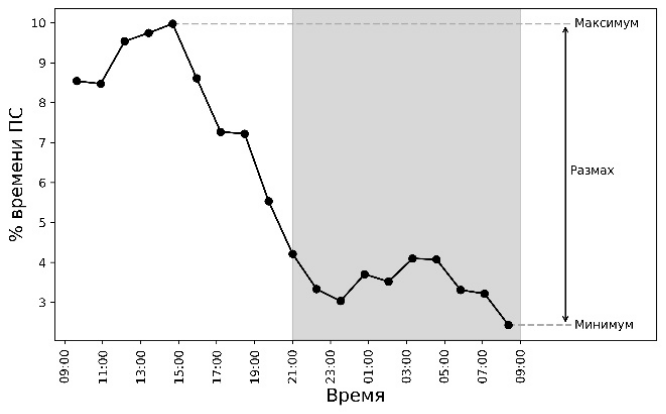
\includegraphics[width=\linewidth]{rem_profile.png}
  \caption{Пример суточного REM-профиля: mean --- уровень;
  размах --- разность max и min.}
\end{figure}

\section{Байесовская модель}

\subsection{Одна разладка}

\[
\mathbf{x}_t\sim
\begin{cases}
p(\mathbf{x}_t\mid\boldsymbol{\theta}_1), & t<\tau,\\
p(\mathbf{x}_t\mid\boldsymbol{\theta}_2), & t\ge\tau,
\end{cases}
\quad
\tau\sim\mathrm{DiscreteUniform}\{3,\ldots,8\}.
\]
$\tau$ маргинализуют из целевой плотности; далее NUTS
(BlackJAX)~\cite{HoffmanGelman2014,lai2023automaticallymarginalizedmcmcprobabilistic}.

\begin{figure}[t]
  \centering
  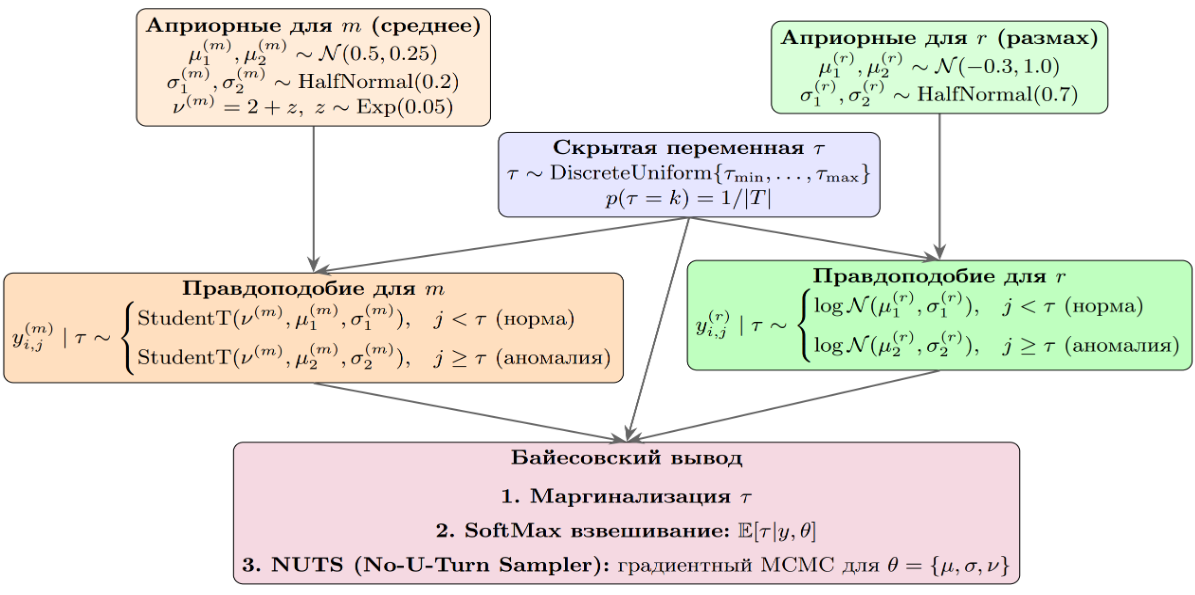
\includegraphics[width=\linewidth]{tau_model.png}
  \caption{Схема: общий $\tau$, отдельные likelihood для mean и range.}
\end{figure}

\subsection{Правдоподобия}

Mean: Student-$t$ (альтернатива normal). Range:
\texttt{beta\_constrained} ($\alpha,\beta\ge 1$ через
\texttt{gamma\_offset}). Plain Beta отвергнут для primary: при
массе $R/2$ у $[0{,}9,1]$ и $\beta{<}1$ PDF взрывается у~$1$,
завышая ELPD~\cite{Vehtari2017}. IIB@$0{,}9$ --- контрольный arm,
не замена A.

\subsection{ELPD / LOO}

PSIS-LOO по парам ``событие--крыса''. Ранжирование ---
$\overline{\elpd}/(F E')$; также $\mathrm{LOO\text{-}IC}=-2\,\elpd$.
Положительный ELPD допустим: continuous densities не вероятности.
Абсолютные ELPD July vs CSV~$896$ без общего builder
\emph{несопоставимы}.

\subsection{Бюджет confirmatory}

tune~$500$, draws~$400$, $2$ цепи, \texttt{nuts\_backend=blackjax},
protocol id \texttt{20260806}. Скрипт
\texttt{run\_integrity\_confirmatory.py}; артефакты
\texttt{run\_output\_integrity\_confirmatory/}.

\section{Результаты Primary~A}

\begin{table}[t]
\centering
\caption{Primary~A и ближайшие контроли (full, $n{=}33$).}
\label{tab:primary-a}
\small
\begin{tabular}{lrrr}
\toprule
Конфиг & $\mathbb{E}[\tau]$ & HDI$_{60}$ & elpd/$FE'$\\
\midrule
\textbf{A:} $t$+constr.\ (24/0.5) & $\mathbf{6{,}285}$ & $1{,}342$ & $3{,}034$\\
A-alt: normal+constr. & $6{,}338$ & $1{,}007$ & $3{,}018$\\
A: $t$+IIB@$0{,}9$ & $7{,}687$ & $0{,}231$ & $2{,}988$\\
mean-only $t$ (24/0.5) & $6{,}043$ & $1{,}835$ & $1{,}807$\\
A при $N{=}48$, ov$0$ & $7{,}356$ & $0{,}463$ & $5{,}258$\\
\bottomrule
\end{tabular}
\end{table}

Основной ответ: onset около \textbf{$6{,}3$ суток} до события.
IIB на том же $(N,\mathrm{ov})$ тянет $\tau$ к верху prior с узким
HDI --- не усреднять с A. Mean-only даёт близкий $\tau$, но хуже
score.

\paragraph{Pareto.}
$\hat k_{\max}{=}0{,}860$; свыше $0{,}7$: R3/before и
R2/after\_reversed на \textbf{$2024$-$09$-$30$}. События оставлены
в primary.

\section{Чувствительность}

\begin{table}[t]
\centering
\caption{Страты для конфига~A (не замена primary).}
\label{tab:sens-a}
\small
\begin{tabular}{lrrr}
\toprule
Страта & $n$ & $\mathbb{E}[\tau]$ & elpd/$FE'$\\
\midrule
full (primary) & $33$ & $6{,}285$ & $3{,}034$\\
drop $2024$-$09$-$30$ & $30$ & $4{,}525$ & $3{,}585$\\
before\_only & $18$ & $3{,}880$ & $3{,}031$\\
\bottomrule
\end{tabular}
\end{table}

$\Delta\mathbb{E}[\tau]\approx -1{,}76$ при дропе влиятельной даты ---
прозрачность, не ``очищенная правда''. Before-only у нижнего края
prior: не смешивать с full при заявлениях о $\tau\approx 6{,}3$.

На сетке чувствительности без plain beta
$\mathbb{E}[\tau]\in[5{,}747;\,7{,}687]$.

\paragraph{Негативный контроль.}
\texttt{shuffle\_dates} (seed~$0$): $\mathbb{E}[\tau]{=}5{,}265$,
HDI$_{60}{=}3{,}625$ (сдвиг к prior); elpd/$FE'{=}3{,}051$ почти как
у real-date --- ELPD-критерий пока слаб; нужны дополнительные семена.

\section{Контекст больших сеток}

В $896$-сетке для Q1 $\mathbb{E}[\tau]{=}6{,}64\pm0{,}42$;
\texttt{concat:mean} доминировал по LOO внутри \emph{той} сетки.
В июле верх часто занимал \texttt{daily:range}+plain~beta --- после
аудита границы это не физиологический ранг. Primary~A намеренно
сочетает уровень и размах на мостовом $(24,0{,}5)$ с density-safe
range-likelihood.

Классическое окно эффекта $2$--$4$\,сут и байесовский onset
$\tau\sim 6{,}3$ --- разные estimand'ы.

\begin{figure}[t]
  \centering
  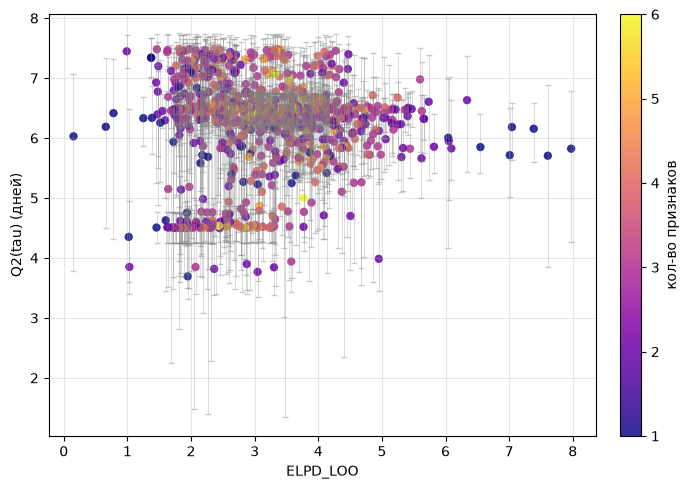
\includegraphics[width=\linewidth]{q2_tau.png}
  \caption{Контекст $896$-сетки: медиана $Q_2(\tau)$ vs ELPD
  (устойчивость onset при вариации ранга).}
\end{figure}

\section{Ограничения}

Выборка мала; одна скачкообразная разладка; artifact-days без
маски в confirmatory builder; RNG seed в сэмплере не прокинут.
Не измеряем кортикостерон / тревогу и не строим прогноз толчков.

\section{Выводы}

\begin{enumerate}[leftmargin=1.2em,itemsep=0.3em]
  \item Primary~A: mean+range, $N{=}24$, $\mathrm{ov}{=}0{,}5$,
  Student-$t$+\texttt{beta\_constrained}, страта full.
  \item $\mathbb{E}[\tau]{=}6{,}285$\,сут; влиятельные окна
  оставлены и задокументированы.
  \item Drop $2024$-$09$-$30$ и before-only --- чувствительность.
  \item Plain Beta --- только диагностика границы; кросс-builder
  ELPD запрещён.
\end{enumerate}

\begin{ack}
Данные --- станция ``Институт''; конвейер \texttt{seismic-pipeline};
цифры --- \texttt{run\_output\_integrity\_confirmatory}.
\end{ack}

{\small
\bibliographystyle{plainnat}
\bibliography{references}
}

\end{document}
